\documentclass[conference,a4paper,flushend]{cs-techrep}
\pdfoutput=1 % pdflatex hint for arxiv.org (within first 5 lines)

\addbibresource{mucLiteratur.bib}
% ======================================================================
% EDIT THESE:

\cstechrepAuthorListTex{Maria Lyoteva, Tsvetan Stanchev}
\cstechrepAuthorListBib{Gruppe 20:, Maria Lyoteva, Tsvetan Stanchev}

% Capitalization: https://capitalizemytitle.com/style/Chicago/
\cstechrepTitleTex{Pulse-Oximeter: Modularbeit für Mobile und Ubiquitous Computing}
 % IF you need manual linebreaks in the titel, then clone the title without linebreaks for BibTeX:
\cstechrepTitleBib{{\cstechrepTitleTex}}


\cstechrepDepartment{Studiengang: Künstliche Intelligenz} % DE
\cstechrepInstitution{Ostbayerische Technische Hochschule Amberg\-/Weiden}
\cstechrepAddress{Amberg, Deutschland} % DE
\cstechrepSeries{Dokumentation der Modularbeit} % DE
\cstechrepYear{2024}
\cstechrepMonth{7}
\cstechrepNumber{\cstechrepYear{}}
\cstechrepLang{ngerman} % DE

% Special remark on babel/csquotes terminology in regard with US-vs-UK:
% en-US  = [english]/[american]/[usenglish] (+ [canadian])
% en-UK  =           [british] /[ukenglish] (+ [australian]) <OXFORD>
% For cs-techrep (like ACM), the recommended english variant is en-US!

% DO NOT DELETE THIS:
\filecontentsForceExpansion|[] % force command expansion inside a filecontents* environment
\begin{filecontents*}[overwrite]{selfref.bib}
    @TECHREPORT{selfref,
        author = {|cstechrepAuthorListBib},
        title  = {\cstechrepTitleBib},
        institution = {\cstechrepInstitution, \cstechrepDepartment},
        series = {\cstechrepSeries},
        number = {\cstechrepNumber},
        year   = {|cstechrepYear},
        month  = {|cstechrepMonth},
        langid  = {|cstechrepLang},
    }
\end{filecontents*}

% ======================================================================
% EDIT THIS:

\begin{filecontents}[overwrite]{embedded.bib}
@online{ieee2015howto,
    author = {Michael Shell},
    title = {How to Use the {IEEEtran} \LaTeX\ Class},
    url = {http://mirrors.ctan.org/macros/latex/contrib/IEEEtran/IEEEtran_HOWTO.pdf},
    year = {2015}
}
@online{ieee2018formattingrules,
    author = {{IEEE}},
    title = {Conference Template and Formatting Specifications},
    url = {https://www.ieee.org/content/dam/ieee-org/ieee/web/org/conferences/Conference-template-A4.doc},
    year = {2018}
}
@online{iaria2014formattingrules,
    author = {{IARIA}},
    title = {Formatting Rules},
    url = {http://www.iaria.org/formatting.doc},
    year = {2014}
}
@online{iaria2009editorialrules,
    _author = {Cosmin Dini},
    author = {{IARIA}},
    title = {Editorial Rules},
    url = {https://www.iaria.org/editorialrules.html},
    year = {2009}
}
@online{languagetool,
    author = {{LanguageTooler GmbH}},
    title  = {{LangueTool}},
    url    = {https://languagetool.org/overleaf}
}
@online{overleaf,
    author = {{Digital Science UK Limited}},
    title  = {{Overleaf}},
    url    = {https://www.overleaf.com}
}
\end{filecontents}

\usepackage{fontawesome} % i.a., \faWarning{}
\usepackage{relsize}     % i.a., \textsmaller{...}
\usepackage{lipsum}      % for blindtext

\usepackage{svg}

\usepackage[table]{xcolor}
\definecolor{lightgray}{gray}{0.8}

\usepackage{dirtree}
\usepackage{multirow}
\usepackage{rotating}
\usepackage{float}
\usepackage{listings}
\usepackage{xcolor}
\usepackage[backend=biber,style=numeric]{biblatex}


\lstset{ 
  language=C++, 
  basicstyle=\ttfamily\small, 
  keywordstyle=\color{blue}, 
  commentstyle=\color{gray}, 
  stringstyle=\color{red}, 
  numbers=left, 
  numberstyle=\tiny\color{gray}, 
  stepnumber=1, 
  numbersep=10pt, 
  backgroundcolor=\color{white}, 
  tabsize=2, 
  captionpos=b, 
  breaklines=true, 
  breakatwhitespace=false, 
  showspaces=false, 
  showstringspaces=false, 
  showtabs=false, 
  frame=single
}

% ======================================================================

% cf. https://ctan.org/pkg/acronym
% Usage:
% singular, within sentence       = \ac{gui}
% singular, beginning of sentence = \Ac{gui}
% plural, within sentence         = \acp{gui}
% plural, beginning of sentence   = \Acp{gui}
\begin{acronym}
    \acro{gui}[GUI]{Graphical User Interface}
    \acro{ide}[IDE]{Integrated Development Environment}
\end{acronym}

% https://www.silbentrennung24.de/
% https://www.hyphenation24.com/
\hyphenation{block-chain block-chains Ethe-re-um}

\begin{document}
\selectlanguage{\cstechrepLang}

\maketitle

\begin{abstract}
Pulse-Oximeter ist eine Android-Anwendung, die den Benutzern die Möglichkeit bietet, ihren Puls und ihre Sauerstoffsättigungswerte zu überwachen. Der Prozess beginnt mit einem \textbf{ESP32-Mikrocontroller, der mit einem MAX30100-Sensor ausgestattet ist}. Dieser sammelt Daten und sendet sie über USB an einen \textbf{PC oder Laptop mit Node-RED}. Node-RED ist für den Empfang, die Aggregation und die Visualisierung dieser Sensordaten zuständig. Die Daten werden dann an einen \textbf{MQTT-Broker} übertragen, der lokal gehostet wird. Schließlich abonniert eine \textbf{Smartphone-App} den MQTT-Broker, um die Daten zu empfangen, sie zu visualisieren und lokal mit SQLite zu speichern. 
\end{abstract}

% A list of IEEE Computer Society approved keywords can be obtained at
% http://www.computer.org/mc/keywords/keywords.htm
\begin{IEEEkeywords}
 ESP32, MAX30100, Node-Red, MQTT, Android.
\end{IEEEkeywords}

%------------------------------

\section{Projektbeschreibung}

\subsection{Einführung}

Im Rahmen der Projektarbeit „Mobile \& Ubiquitous Computing“ wird eine Biosensor-App entwickelt, die Echtzeitdaten eines Herzfrequenz- und Pulsoximetersensors (MAX30100) erfasst und visualisiert. Die App nutzt die Möglichkeiten des  IoT („Internet of Things“), um Sensordaten zu aggregieren, zu visualisieren und für die spätere Analyse zu speichern.

\subsection{Ziele des Projekts}

Die primären Ziele dieses Projekts sind:
\begin{itemize}
    \item \textbf{Sensor Data Acquisition}: Echtzeitdaten eines optischen Herzfrequenz- und Pulsoximetersensors (MAX30100) mit einem ESP32-Mikrocontroller erfassen.
    \vspace{0.5em}
    \item \textbf{Data Aggregation and Visualization}: Aggregation und Visualisierung der Sensordaten mit Node-RED und Veröffentlichung über das MQTT-Protokoll.
    \vspace{0.5em}
    \item \textbf{Mobile Application Development}: Entwicklung einer Android-Anwendung zur Anzeige und Speicherung der Sensordaten.
\end{itemize}

\subsection{Architektur des Projekts}

Die Architektur des Projekts umfasst vier Hauptkomponenten:
\begin{itemize}
    \item \textbf{ESP32 Microcontroller mit MAX30100 Sensor}:
    \begin{itemize}
        \item Der MAX30100 Sensor ist über die I2C-Schnittstelle mit dem ESP32 Mikrocontroller verbunden, welcher die Herzfrequenz und die Blutsauerstoffsättigung erfasst und die Daten über eine serielle USB-Verbindung an einen PC oder Laptop sendet.
    \end{itemize}
    \item \textbf{PC/Laptop mit Node-RED}:
    \begin{itemize}
        \item Node-RED liest die Sensordaten vom ESP32, verarbeitet und visualisiert sie. Die Daten werden anschließend über das MQTT-Protokoll veröffentlicht.
    \end{itemize}
    \item \textbf{MQTT Broker}:
    \begin{itemize}
        \item Der MQTT-Broker (lokal oder cloudbasiert) dient als Vermittler für die Datenkommunikation zwischen Node-RED und der mobilen Anwendung.
    \end{itemize}
    \item \textbf{Smartphone Anwendung}:
    \begin{itemize}
        \item Die mobile Anwendung empfängt die Sensordaten vom MQTT-Broker, zeigt sie in einem benutzerfreundlichen Dashboard an und speichert sie lokal in einer SQLite-Datenbank.
    \end{itemize}
\end{itemize}


\section{Funktionsweise des Sensors}

\subsection{Einführung in den MAX30100-Sensor}

Der MAX30100 ist ein integrierter Pulsoximeter- und Herzfrequenzsensor, der für tragbare Gesundheitsanwendungen entwickelt wurde. Der Sensor misst die Sauerstoffsättigung im Blut (SpO2) und die Herzfrequenz (HR) durch die Analyse der Lichtabsorption bei verschiedenen Wellenlängen.

\subsection{Funktionsprinzip}

Der MAX30100-Sensor arbeitet, indem er Licht durch das Gewebe sendet und die Lichtintensität misst, die auf der anderen Seite empfangen wird. Zwei LEDs, eine rote und eine infrarote, werden abwechselnd eingeschaltet, und ein Photodetektor misst das durch den Finger hindurchgelassene Licht. Durch die Analyse der Lichtabsorption bei den beiden verschiedenen Wellenlängen kann der Sensor die SpO2 und die HR bestimmen.

\subsection{Sensorbetrieb}

\begin{itemize}
    \item \textbf{LEDs und Photodetektor}: Die rote LED und die infrarote LED senden Licht durch das Gewebe, und der Photodetektor misst das durchgelassene Licht.
    \vspace{0.5em}
    \item \textbf{Datenanalyse}: Der Sensor analysiert die Lichtabsorption, um die SpO2 und die HR zu bestimmen.
    \vspace{0.5em}
    \item \textbf{Datenübertragung}: Die erfassten Daten werden über die I2C-Schnittstelle an den ESP32 Mikrocontroller übertragen.
\end{itemize}

\subsection{Vorteile und Einschränkungen}

\begin{itemize}
    \item \textbf{Vorteile}: Hohe Genauigkeit, Echtzeitmessungen, geringe Größe und Energieverbrauch.
    \item \textbf{Einschränkungen}: Empfindlichkeit gegenüber Bewegungsartefakten, Lichtinterferenzen und Hautpigmentierungen.
\end{itemize}

\section{Projektplanung und Vorgehen}

\subsection{Teamaufteilung}

Die Teamaufteilung erfolgte wie folgt:
\begin{table}[h!]
    \centering
    \renewcommand{\arraystretch}{2} % Adjust this value to increase/decrease row height
    \begin{tabular}{|p{3cm}|p{5cm}|}
        \hline
        \textbf{Aufgabe} & \textbf{Verantwortlich} \\ \hline
        Zusammenbau der Hardware & Tsvetan \\ \hline
        Arduino Code & Tsvetan \\ \hline
        Vorbereitung des Mosquitto Brokers & Maria \\ \hline
        Erstellung des Node-Red-Flows & Tsvetan und Maria \\ \hline
        Frontend & Maria \\ \hline
        \multirow{2}{3cm}{Backend} & Maria: MainActivity, MqttData, MqttManager, SoundManager \\ 
                                   & Tsvetan: OptionsActivity, DataTableActivity, DataAdapter, DatabaseHelper, ChartManager \\ \hline
        Dokumentation & Tsvetan und Maria \\ \hline
    \end{tabular}
    \vspace{0.5cm} % Add vertical space before the caption
    \caption{Projektaufgaben und Verantwortlichkeiten}
    \label{tab:project_tasks}
\end{table}
\vspace{10em}
\subsection{Zeitleiste}

Ein detaillierter Zeitplan, der die wichtigsten Meilensteine und Aufgaben darstellt:
\begin{table}[H]
    \centering
    \renewcommand{\arraystretch}{2} % Adjust this value to increase/decrease row height
    \begin{tabular}{|c|l|}
        \hline
        \textbf{Woche} & \textbf{Aufgabe} \\ \hline
        1-2 & Hardware-Setup und Sensorintegration \\ \hline
        3-4 & Node-RED Konfiguration und Datenvisualisierung \\ \hline
        5-6 & Entwicklung der Smartphone-App \\ \hline
        7-8 & Testing, Debugging und Dokumentation \\ \hline
    \end{tabular}
    \vspace{0.5cm} % Add vertical space before the caption
    \caption{Zeitplan}
    \label{tab:zeitleiste}
\end{table}

\section{Projektimplementierung}
\subsection{Hardware-Konfiguration}
\subsubsection{Hardware-Komponenten}
Wir haben die folgenden Komponenten verwendet:
\vspace{0.5em}
\begin{itemize}
    \item \textbf{ESP32 Mikrocontroller}: Ein leistungsfähiger Mikrocontroller mit WLAN- und Bluetooth-Fähigkeiten.
    \vspace{0.5em}
    \item \textbf{MAX30100 Sensor}: Ein integrierter Pulsoximeter- und Herzfrequenzsensor.
    \vspace{0.5em}
    \item \textbf{Breadboard}: Ein Steckbrett zur Herstellung von provisorischen Schaltungen ohne Löten.
    \vspace{0.5em}
    \item \textbf{Verbindungskabel}: Verschiedene farbige Jumper-Kabel zur Verbindung der Komponenten.
    \end{itemize}
\vspace{0.8em}
\subsubsection{Verkabelung}
 Die Konfiguration der Verbindungen wurde wie folgt vorgenommen:
\begin{itemize}
    \item \textbf{VIN} des Sensors wurde mit dem \textbf{3.3V} Pin des ESP32 verbunden (braune Leitung). Dies versorgt den Sensor mit der notwendigen Betriebsspannung.
    \vspace{0.5em}
    \item \textbf{GND} des Sensors wurde mit dem \textbf{GND} Pin des ESP32 verbunden (rote Leitung). Dies stellt die gemeinsame Masseverbindung her.
    \vspace{0.5em}
    \item \textbf{SCL} des Sensors wurde mit dem \textbf{Port 33} Pin des ESP32 verbunden (orange Leitung). Dies ist die serielle Taktleitung für die I2C-Kommunikation.
    \vspace{0.5em}
    \item \textbf{SDA} des Sensors wurde mit dem \textbf{Port 32} Pin des ESP32 verbunden (gelbe Leitung). Dies ist die serielle Datenleitung für die I2C-Kommunikation.
\end{itemize}
\vspace{0.5em}
Abbildung \ref{fig:hardware} zeigt ein Beispiel der Hardware-Konfiguration auf einem Breadboard, welches die oben beschriebenen Verbindungen veranschaulicht:

\begin{figure}[h]
    \centering
    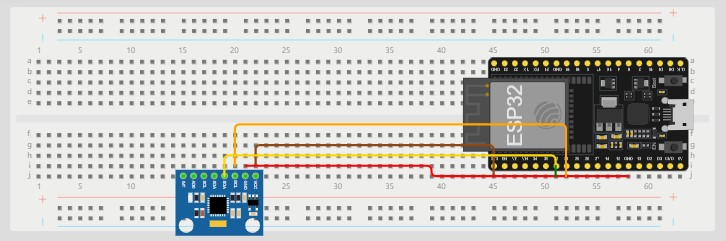
\includegraphics[width=0.45\textwidth]{hardware-config.jpg}
    \caption{Hardware-Konfiguration des ESP32 und MAX30100 Sensors auf einem Breadboard}
    \label{fig:hardware}
\end{figure}

\subsection{Verarbeitung der Sensor-Daten}

\subsubsection{Programmierung des ESP32 mit der Arduino IDE}
Der ESP32 Mikrocontroller wird mit der Arduino IDE programmiert, um die Herzfrequenz- (BPM) und Sauerstoffsättigungsdaten (SpO2) zu erfassen.
\vspace{0.5em}

\subsubsection{Einbindung der Bibliotheken}
Es werden die \textbf{Wire}- und \textbf{MAX30100\_PulseOximeter}-Bibliotheken eingebunden, die für die Kommunikation mit dem MAX30100-Sensor erforderlich sind.
\vspace{0.5em}
\begin{lstlisting}
#include <Wire.h>
#include "MAX30100_PulseOximeter.h"
\end{lstlisting}

\subsubsection{Initialisierung des Sensors}
Der Sensor wird über die I2C-Schnittstelle (SDA zu GPIO 33, SCL zu GPIO 32) initialisiert. Falls die Initialisierung fehlschlägt, bleibt der ESP32 in einer Endlosschleife hängen.
\vspace{0.5em}
\begin{lstlisting}
    void setup()
{
  Serial.begin(9600);
  Serial.println("Initializing pulse oximeter..");

  Wire.begin(32, 33);  // Initialize I2C with custom pins if necessary (SDA to GPIO 33, SCL to GPIO 32)

  if (!pox.begin()) {
    Serial.println("FAILED to initialize pulse oximeter");
    while (1);  // Hang indefinitely if initialization fails
  } else {
    Serial.println("Pulse oximeter initialized successfully");
  }

  pox.setOnBeatDetectedCallback(onBeatDetected);
}
\end{lstlisting}

\subsubsection{Herzschlag-Erkennung}
Wenn ein Herzschlag erkannt wird, wird das pulseDetected-Flag gesetzt.
\vspace{0.5em}
\begin{lstlisting}
    void onBeatDetected() {
    pulseDetected = true; // Set flag when a beat is detected
}
\end{lstlisting}
%\clearpage
\subsubsection{Datenverarbeitung}
Die Herzfrequenz- und SpO2-Werte werden über einen Zeitraum von 10 Sekunden gemessen und akkumuliert. Anschließend wird der Durchschnitt berechnet und über die serielle Schnittstelle ausgegeben.
\vspace{0.5em}
\begin{lstlisting}
    void loop() {

  pox.update();

  if (pulseDetected) {

    if (startTime == 0) {
      startTime = millis(); // Start timing
    }

    elapsedTime = millis() - startTime;

    if (elapsedTime < 1000) { // 10 seconds in milliseconds
      // Accumulate heart rate and SpO2
      heartRateSum += pox.getHeartRate();
      spo2Sum += pox.getSpO2();
      measurementsNumber += 1;
    } else {
      Serial.print(heartRateSum / measurementsNumber); // Average heart rate over 10 seconds
      Serial.print(",");
      Serial.println(spo2Sum / measurementsNumber); // Average SpO2 over 10 seconds
      
      // Reset variables for the next 10-second interval
      startTime = 0;
      elapsedTime = 0;
      heartRateSum = 0;
      spo2Sum = 0;
      measurementsNumber = 0;
      pulseDetected = false;
    }
  }
}
\end{lstlisting}

\subsection{Node-Red Konfiguration und Datenvisualisierung- I Stufe}
Unser Node-RED-Flow simuliert die Erfassung von Herzfrequenz- und Sauerstoffsättigungsdaten durch die Verwendung von zufällig generierten Werten. Die generierten Herzfrequenzwerte liegen im Bereich von 60 bis 80 BPM, während die Sauerstoffsättigungswerte im Bereich von 90 bis 98 Prozenten liegen. Diese Simulation ermöglicht eine einfache und effektive Testumgebung, ohne dass echte Sensoren benötigt werden. Die generierten Daten werden in Echtzeit über MQTT an das Dashboard gesendet, wo sie visualisiert werden können. In den nächsten Schritten werden wir unseren Flow im Detail erklären.
\vspace{0.5em}
\begin{figure}[H]
    \centering
    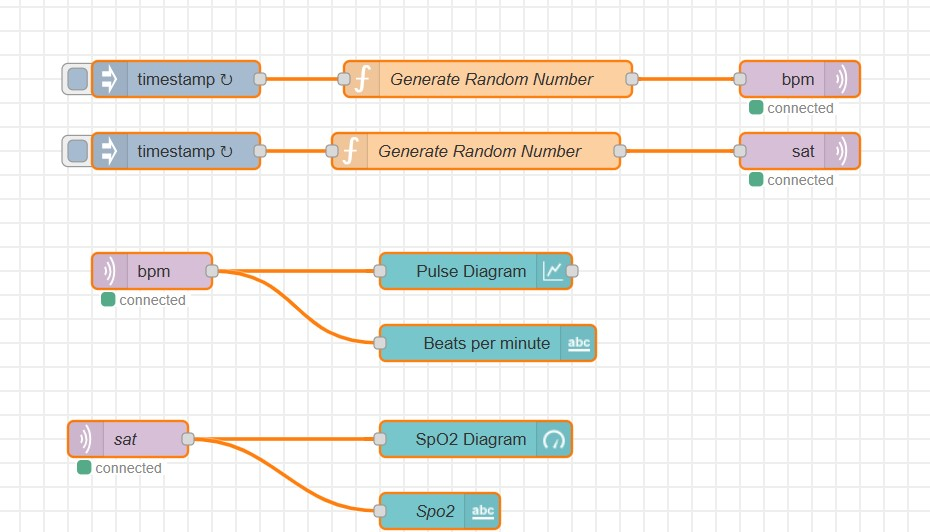
\includegraphics[width=0.48\textwidth]{dummy_flow.jpg}
    \caption{Node-RED Flow zur Simulation von Herzfrequenz- und Sauerstoffsättigungsdaten}
    \label {fig:flow}
\end{figure}

\subsubsection{Injektionsknoten}
Der Flow beginnt mit zwei Injektionsknoten, die in regelmäßigen Abständen Nachrichten auslösen. Diese Knoten senden initiale Nachrichten, die zur Generierung der Zufallsdaten dienen.
\begin{itemize}
\vspace{0.5em}
\item\textbf {inject\_node}
Dieser Knoten sendet jede Sekunde eine Nachricht. Die Nachricht wird an den Funktionsknoten weitergeleitet, der zufällige BPM-Werte generiert.
\vspace{0.5em}
\item\textbf {inject\_node\_2} 
Dieser Knoten sendet ebenfalls jede Sekunde eine Nachricht. Die Nachricht wird an den zweiten Funktionsknoten weitergeleitet, der zufällige SpO2-Werte generiert.
\vspace{0.5em}
\end{itemize}

\subsubsection{Funktionsknoten}
Die Funktionsknoten sind so programmiert, dass sie zufällige Werte innerhalb eines bestimmten Bereichs generieren und diese an die entsprechenden MQTT-Ausgabeknoten senden.
\begin{itemize}
\vspace{0.5em}
\item\textbf {function\_node (Generate Random Number)}\\
Dieser Knoten generiert eine zufällige Herzfrequenz (BPM) im Bereich von 60 bis 80. Der erzeugte Wert wird dann an den MQTT-Ausgabeknoten gesendet.
\vspace{0.5em}
\item\textbf {function\_node\_2 (Generate Random Number)}\\
Dieser Knoten generiert eine zufällige Sauerstoffsättigung (SpO2) im Bereich von 90 bis 98. Der erzeugte Wert wird dann an den MQTT-Ausgabeknoten gesendet. 
\vspace{0.5em}
\end{itemize}

\subsubsection{MQTT-Ausgabeknoten}
Die MQTT-Ausgabeknoten senden die generierten Daten an die MQTT-Broker, von wo aus sie an die entsprechenden MQTT-Eingabeknoten weitergeleitet werden.
\begin{itemize}
\item\textbf {mqtt\_out\_node}\\
Sendet die generierten BPM-Daten an das MQTT-Thema "bpm".
\vspace{0.5em}
\item\textbf {mqtt\_out\_node\_2}\\
Sendet die generierten SpO2-Daten an das MQTT-Thema "sat". ("sat" steht für "saturation")
\vspace{0.5em}
\end{itemize}

\subsubsection{MQTT-Eingabeknoten}
Die MQTT-Eingabeknoten empfangen die Daten von den MQTT-Brokern und leiten diese an die Dashboard-Knoten weiter.
\begin{itemize}
\vspace{0.5em}
\item\textbf{mqtt\_in\_node (BPM):}\\
Empfängt die BPM-Daten vom MQTT-Thema "bpm" und sendet sie an das Diagramm und den Textanzeige-Knoten.
\vspace{0.5em}
\item\textbf{mqtt\_in\_node\_2 (SpO2):}
Empfängt die SpO2-Daten vom MQTT-Thema "sat" und sendet sie an das Gauge-Diagramm und den Textanzeige-Knoten.
\vspace{0.5em}
\end{itemize}

\subsubsection{Dashboard-Knoten}
Die Dashboard-Knoten visualisieren die empfangenen Daten. Dies ermöglicht eine einfache Überwachung der simulierten Werte.
\begin{itemize}
\vspace{0.5em}
\item\textbf{ui\_chart}: Zeigt die BPM-Daten in einem Liniendiagramm an. Dies ermöglicht die visuelle Verfolgung der Herzfrequenz über die Zeit.
\vspace{0.5em}
 \item\textbf{ui\_text}: Zeigt die BPM-Daten als Text an. Dies bietet eine klare und präzise Anzeige der aktuellen Herzfrequenz.
 \vspace{0.5em}
 \item\textbf{ui\_text\_2}: Zeigt die SpO2-Daten als Text an. Dies bietet eine klare und präzise Anzeige der aktuellen Sauerstoffsättigung.
 \vspace{0.5em}
 \item\textbf{ui\_gauge}: Zeigt die SpO2-Daten in einem Gauge-Diagramm an. Dies bietet eine schnelle visuelle Rückmeldung über die Sauerstoffsättigung.
\vspace{0.5em}
\end{itemize}

\subsubsection{Dashboard Visualisierung und Erklärung}
Sie können unser Dashboard auf dem untenstehenden Bild sehen:
\begin{figure}[H]
    \centering
    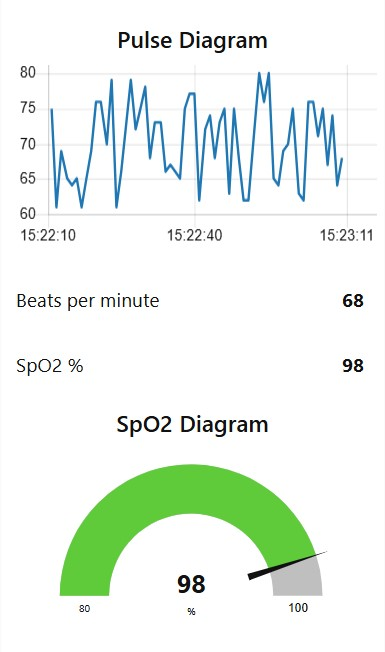
\includegraphics[width=0.4\textwidth]{dash_node_green.jpg}
    \caption{Node-Red Dashboard}
    \label{fig:dashboard}
\end{figure}
Das Gauge-Diagramm, das die SpO2-Daten anzeigt, verwendet verschiedene Farben, um unterschiedliche Bereiche der Sauerstoffsättigung im Blut darzustellen:


\begin{itemize}
    \item\textbf{Grün - Normaler Bereich:} 95\% bis 100\% - Dieser Bereich zeigt eine gute Sauerstoffversorgung des Blutes und der Organe an. (Abbildung 3)
    \vspace{0.5em}
    \item\textbf{Gelb - Leichte Hypoxie}
    90\% bis 94\% - Werte in diesem Bereich können auf eine leichte Beeinträchtigung der Sauerstoffversorgung hinweisen und sollten überwacht werden. (Abbildung 4) 
    \vspace{0.5em}
    \begin{figure}[H]
    \centering
    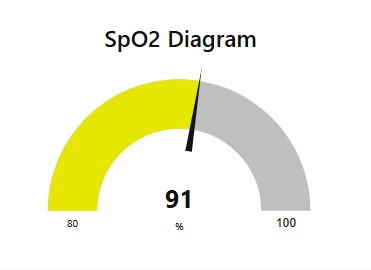
\includegraphics[width=0.4\textwidth]{dash_yellow.jpg}
    \caption{Gauge-Diagramm gelb}
    \label{fig:dash_yellow}
    \end{figure}
    \item\textbf{Rot - Schwere Hypoxie}
    Unter 90\% - Werte unter 90\% sind besorgniserregend und erfordern sofortige medizinische Intervention. (Abbildung 5)
    \begin{figure}[H]
    \centering
    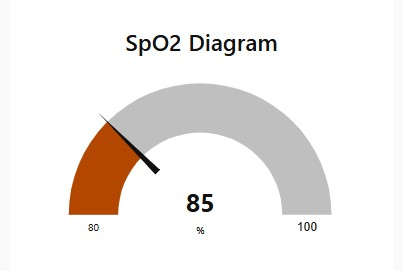
\includegraphics[width=0.4\textwidth]{dash_red.jpg}
    \caption{Gauge-Diagramm rot}
    \label{fig:dash_ed}
    \end{figure}
\end{itemize}

\subsection{Node-Red Konfiguration und Datenvisualisierung- II Stufe}
Dieser Node-RED-Flow(Abbildung 6) dient der Verarbeitung und Visualisierung von Herzfrequenz- (BPM) und Sauerstoffsättigungsdaten (SpO2). Daten werden über eine serielle Schnittstelle empfangen, aufgeteilt und dann über MQTT an ein Dashboard zur Visualisierung gesendet.
\begin{figure}[h]
    \centering
    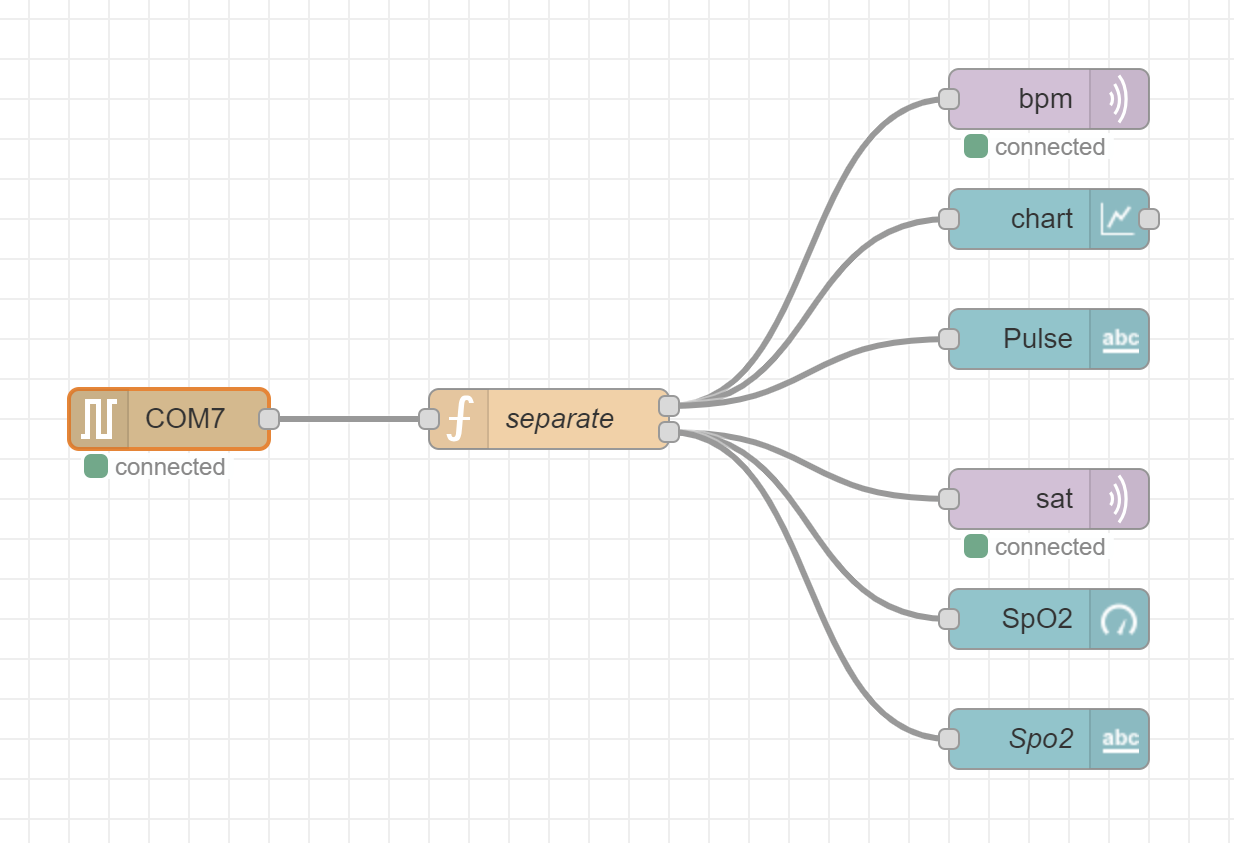
\includegraphics[width=0.4\textwidth]{dash_2.png}
    \caption{Node-Red Flow mit den realen Daten}
    \label{fig:dashboard2}
\end{figure}

\subsubsection{Injektionsknoten}
Der Flow beginnt mit dem Empfang von Daten über eine serielle Schnittstelle.
(COM7 von unserem PC)

\subsubsection{Funktionsknoten}
Der Funktionsknoten sind so programmiert, dass sie die empfangenen Daten in zwei getrennte Nachrichten aufteilen, eine für BPM und eine für SpO2.
\begin{figure}[h]
    \centering
    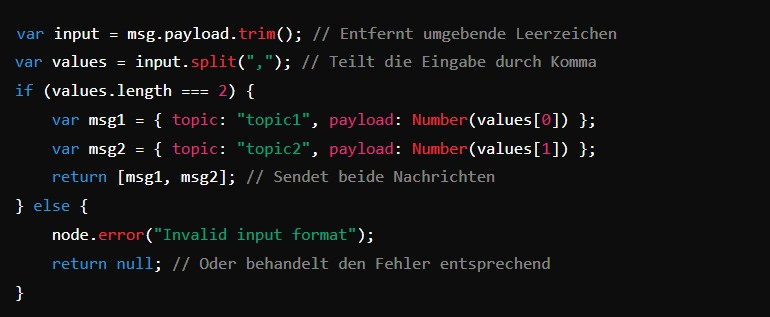
\includegraphics[width=0.5\textwidth]{funktionsknoten_code.jpg}
    \caption{Funktionimplementierung}
    \label{fig:funktionsnknoten-code}
\end{figure}

\subsubsection{MQTT- und Dashboard- Knoten}
Die MQTT- und Dashboard-Knoten arbeiten nach dem gleichen Prinzip wie diejenigen im ersten Flow. 

\subsection{MQTT Konfiguration}
\subsubsection{Einleitung}
MQTT (Message Queuing Telemetry Transport) ist ein leichtes Protokoll für die Nachrichtenübermittlung, das häufig in IoT-Anwendungen (Internet of Things) verwendet wird. In unserem Projekt haben wir MQTT lokal installiert und verwenden es zur Kommunikation zwischen verschiedenen Geräten, einschließlich des ESP32-Mikrocontrollers und einer Android-App im Emulator. Zusätzlich nutzen wir MQTTX, um die Datenübertragung zu überprüfen und sicherzustellen, dass die Nachrichten korrekt gesendet und empfangen werden.

\subsubsection{Installation und Konfiguration des MQTT-Brokers}
Wir haben einen MQTT-Broker lokal auf unseren PCs installiert, um als zentraler Kommunikationsknotenpunkt zu dienen. Der Broker verwendet den Standardport 1883 und ist so konfiguriert, dass er Nachrichten von verschiedenen MQTT-Clients empfängt und verteilt. \vspace{0.5em}

\subsubsection{Verwendung von MQTTX zur Überprüfung der Datenübertragung}
MQTTX ist ein MQTT 5.0 Desktop-Client, der uns ermöglicht, die MQTT-Kommunikation zu testen und zu überwachen. Wir verwenden MQTTX, um sicherzustellen, dass die Daten, die vom ESP32 gesendet werden, korrekt empfangen und verarbeitet werden. \vspace{0.5em}

\underline {Verbindung zum MQTT-Broker herstellen:}
     \begin{itemize}
         \vspace{0.5em}
         \item Starten Sie MQTTX und fügen Sie eine neue Verbindung hinzu.
         \begin{figure}[H]
         \centering
         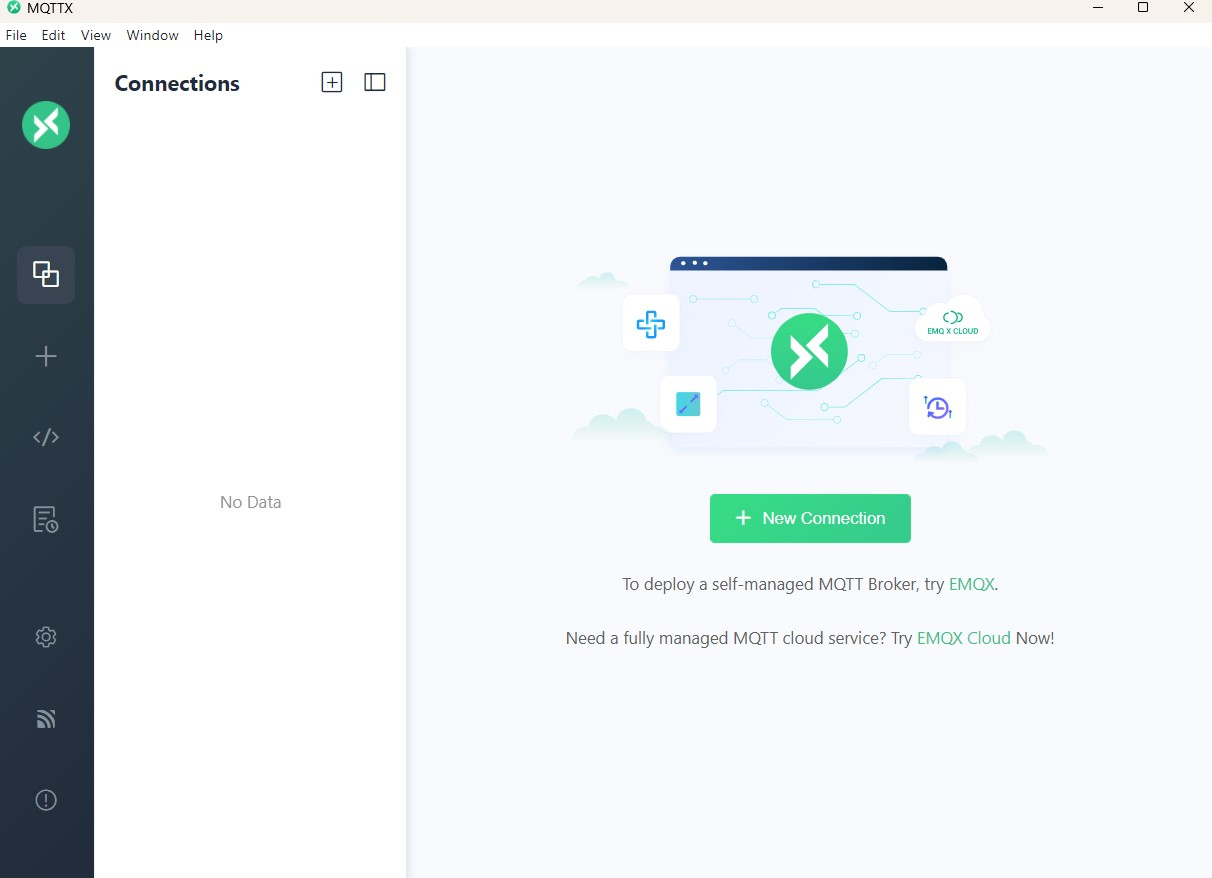
\includegraphics[width=0.4\textwidth]{MQTTX_Start.jpg}
         \caption{MQTTX Homescreen}
         \label{fig:funktionsnknoten-code}
         \end{figure}
         \vspace{0.5em}
         \item Geben Sie die Broker-Adresse (localhost) und den Port (1883) ein.
         \vspace{0.5em}
         \begin{figure}[H]
         \centering
         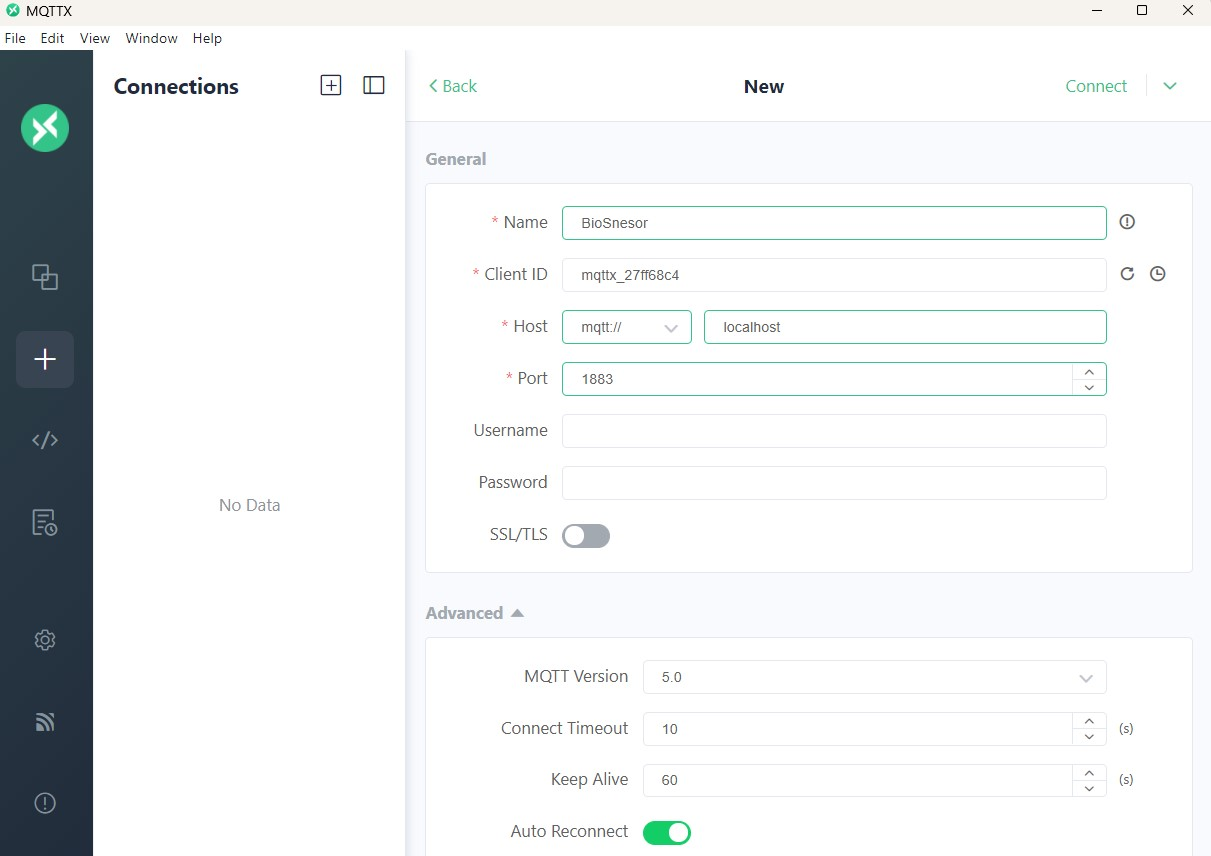
\includegraphics[width=0.4\textwidth]{mqttx_new_connection.jpg}
         \caption{neue Verbindung erstellen}
         \label{fig:funktionsnknoten-code}
         \end{figure}
         \item Klicken Sie auf "Connect", um die Verbindung zum lokalen MQTT-Broker herzustellen.
         \vspace{0.5em}
     \end{itemize}

\underline{Überprüfen der Datenübertragung:} 
     \begin{itemize}
         \vspace{0.5em}
         \item Abonnieren Sie die Themen bpm und sat, um die empfangenen Daten anzuzeigen.
         \begin{figure}[h]
         \centering
         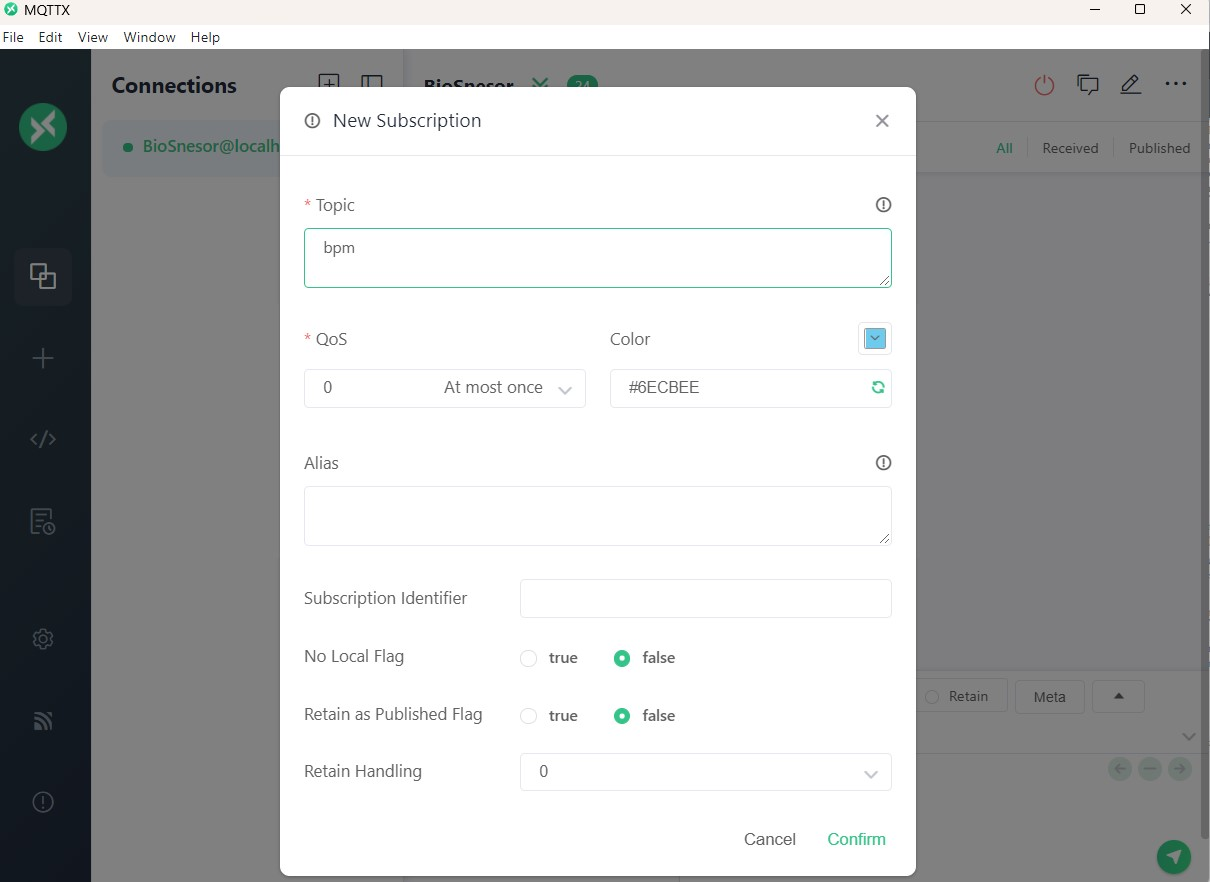
\includegraphics[width=0.4\textwidth]{subscribe_bpm.jpg}
         \caption{Themen (Topics) abonnieren}
         \label{fig:funktionsnknoten-code}
         \end{figure}
         \item Die Verbindung überprüfen. 
         \begin{figure}[h]
         \centering
         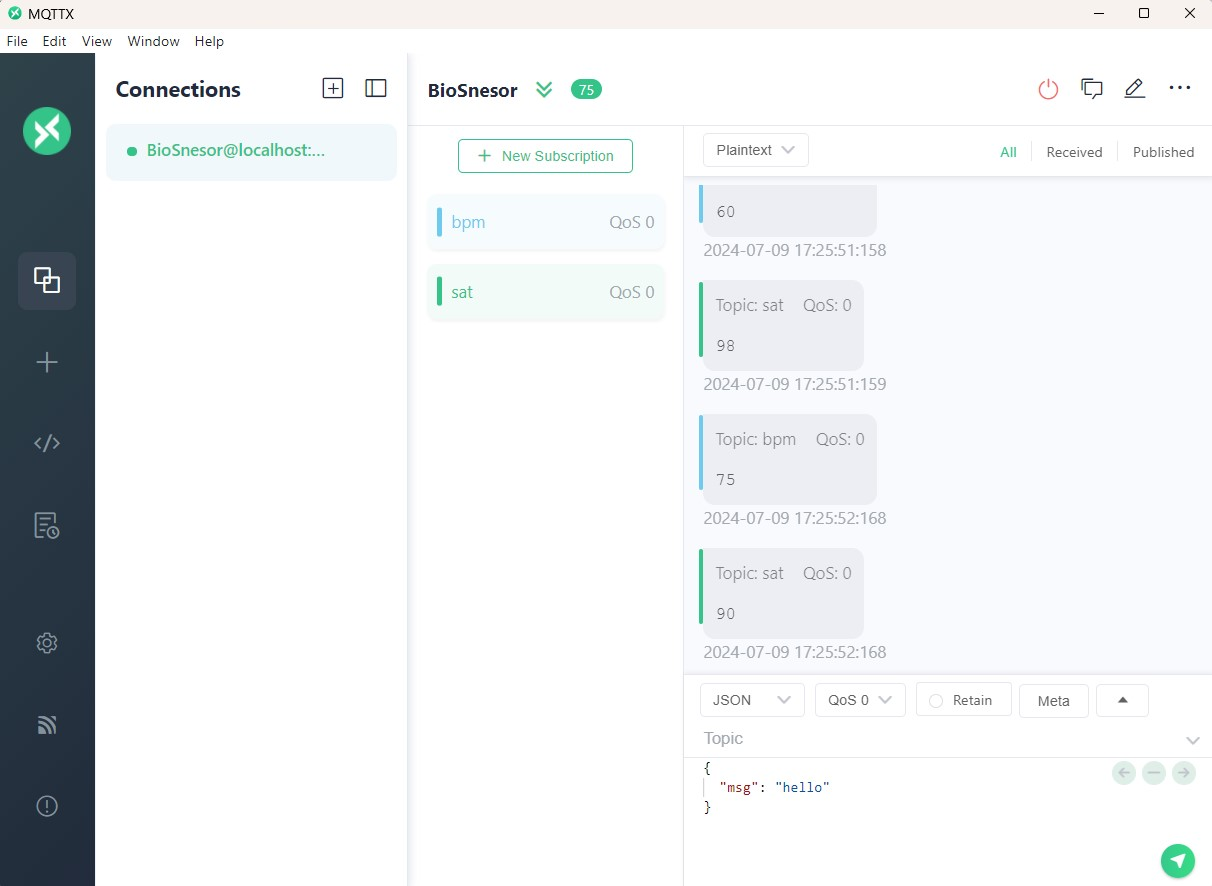
\includegraphics[width=0.4\textwidth]{daten_bpm_sat.jpg}
         \caption{Daten visualizieren}
         \label{fig:funktionsnknoten-code}
         \end{figure}
     \end{itemize}

\subsection{Entwicklung der Smartphone App}
Wir haben uns entschieden, eine Android-App zu entwickeln, die in einem Android Studio Emulator (Pixel 7, API27 Device) läuft. Unser Projekt ist eine Android-Anwendung zur Überwachung und Anzeige von Herzfrequenz- und Sauerstoffsättigungdaten. Es verwendet MQTT, um Echtzeitdaten zu empfangen, speichert diese Daten in einer lokalen Datenbank und bietet Funktionen zur Ansicht und Verwaltung der Daten über verschiedene UI-Komponenten und Aktivitäten. 
\vspace{0.5em}\\
\underline{Emulator in Android Studio konfigurieren}
\vspace{0.2em}

Um einen Emulator für ein Pixel 7 mit API 27 zu konfigurieren, folgen Sie diesen Schritten:
\vspace{0.5em}
\begin{enumerate}
    \item \textbf{Android Studio öffnen:} \\
    Öffnen Sie Android Studio auf Ihrem Computer.
    
    \item \textbf{AVD Manager öffnen:}
    \begin{itemize}
        \item Klicken Sie in der Menüleiste auf \texttt{Tools}.
        \vspace{0.5em}
        \item Wählen Sie \texttt{AVD Manager} aus dem Dropdown-Menü oder klicken Sie auf das AVD Manager-Symbol in der Symbolleiste.
        \vspace{0.5em}
    \end{itemize}
    \vspace{0.5em}
    \item \textbf{Neues virtuelles Gerät erstellen:}
    \begin{itemize}
        \item Klicken Sie im AVD Manager auf \texttt{Create Virtual Device}.
        \vspace{0.5em}
        \item Wählen Sie \texttt{Pixel 7} aus der Liste der verfügbaren Geräte.
        \vspace{0.5em}
        \item Klicken Sie auf \texttt{Next}.
        \vspace{0.5em}
    \end{itemize}
    \vspace{0.5em}
    \item \textbf{Systemabbild auswählen:}
    \begin{itemize}
        \item Wählen Sie die Android-Version \texttt{API 27} aus.
        \vspace{0.5em}
        \item Wenn das Systemabbild nicht verfügbar ist, klicken Sie auf 
        \vspace{0.5em}
        \texttt{Download} und installieren Sie es.
        \vspace{0.5em}
        \item Klicken Sie auf \texttt{Next}.
        \vspace{0.5em}
    \end{itemize}
    \vspace{0.5em}
    \item \textbf{AVD-Einstellungen konfigurieren:}
    \vspace{0.5em}
    \begin{itemize}
        \item Geben Sie Ihrem virtuellen Gerät einen Namen im Feld \texttt{AVD Name}.
        \vspace{0.5em}
        \item Überprüfen Sie die restlichen Einstellungen und passen Sie sie nach Bedarf an.
        \vspace{0.5em}
        \item Klicken Sie auf \texttt{Finish}, um das virtuelle Gerät zu erstellen.
        \vspace{0.5em}
    \end{itemize}
    \vspace{0.5em}
    \item \textbf{Virtuelles Gerät starten:}
    \vspace{0.5em}
    \begin{itemize}
        \item Finden Sie Ihr neu erstelltes virtuelles Gerät in der Liste der verfügbaren AVDs im AVD Manager.
        \vspace{0.5em}
        \item Klicken Sie auf das grüne Wiedergabe-Symbol (\texttt{Launch this AVD in the emulator}), um das virtuelle Gerät zu starten.
        \vspace{0.5em}
    \end{itemize}
    \vspace{0.5em}
    \item \textbf{Anwendung auf dem Emulator ausführen:}
    \vspace{0.5em}
    \begin{itemize}
        \item Öffnen Sie Ihr Projekt in Android Studio.
        \vspace{0.5em}
        \item Wählen Sie das neu gestartete virtuelle Gerät aus der Dropdown-Liste in der Symbolleiste aus (neben dem grünen \texttt{Run}-Button).
        \vspace{0.5em}
        \item Klicken Sie auf den \texttt{Run}-Button (grünes Dreieck), um Ihre Anwendung auf dem Emulator auszuführen.
        \vspace{0.5em}
    \end{itemize}
\end{enumerate}
\subsubsection{Frontend}
Die Benutzeroberfläche der Pulsoximeter-App besteht aus mehreren Seiten, die verschiedene Funktionen und Informationen darstellen.

\underline{Hauptseite}\vspace{0.5em}\\
Der Hauptbildschirm zeigt die aktuellen Messwerte des Pulsoximeters sowie Steuerungselemente für die Messung.

 \begin{figure}[h]
         \centering
         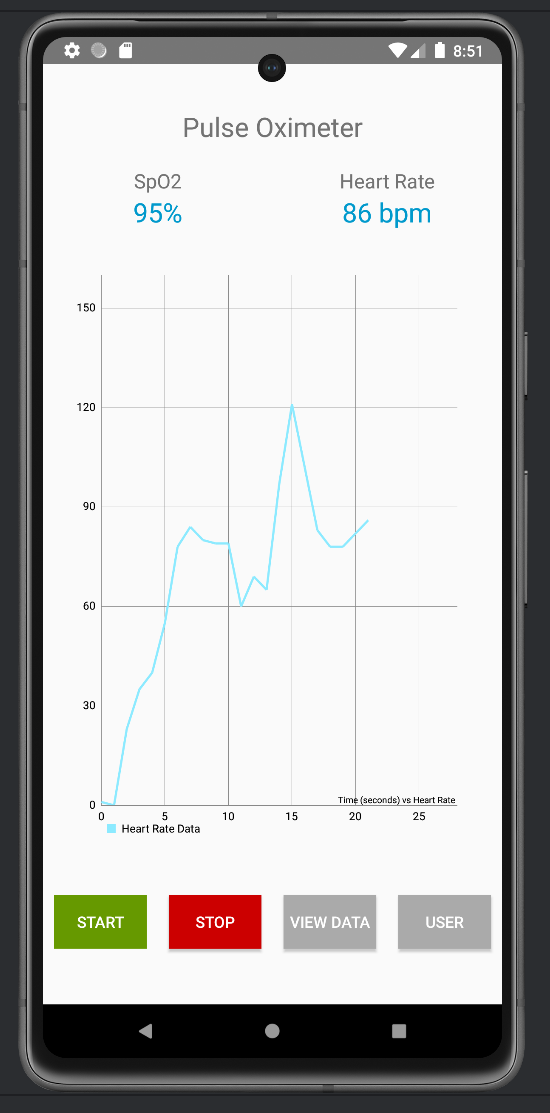
\includegraphics[width=0.4\textwidth]{final_app.png}
         \caption{Datenanzeigeseite}
         \label{fig:finalApp}
 \end{figure}
\textbf{Hauptverantwortlichkeiten:}
\begin{itemize}
    \vspace{0.5em}
    \item \textbf{Titel TextView:} Zeigt den Titel "Pulsoximeter" zentriert auf dem Bildschirm an. Der Titel hat eine Textgröße von 24sp und ist horizontal zentriert mit einem oberen Randabstand von 40dp.
    \vspace{0.5em}
    \item \textbf{Anzeigebereich: SpO2 und Herzfrequenz:} Enthält zwei vertikale Layouts für die Anzeige von SpO2 (Sauerstoffsättigung) und Herzfrequenz. Der Anzeigebereich ist horizontal zentriert unterhalb des Titels mit einem oberen Randabstand von 20dp.
    \vspace{0.5em}
    \begin{itemize}
        \item \textbf{SpO2-Anzeige:} Zeigt den Text "SpO2" an und die aktuelle SpO2-Messung (Standardanzeige: "--"). Die Textfarbe ist dunkelblau und die Textgröße beträgt 24sp.
        \vspace{0.5em}
        \item \textbf{Herzfrequenz-Anzeige:} Zeigt den Text "Herzfrequenz" an und die aktuelle Herzfrequenz-Messung (Standardanzeige: "--"). Die Textfarbe ist dunkelblau und die Textgröße beträgt 24sp.
    \end{itemize}
    \vspace{0.5em}
    \item \textbf{Liniendiagramm:} Zeigt ein Liniendiagramm der Herzfrequenzdaten an. Das Diagramm füllt die Breite des Bildschirms aus und befindet sich unterhalb des Anzeigebereichs und oberhalb der Steuerelemente mit Randabständen von 25dp oben, links und rechts.
    \vspace{0.5em}
    \item \textbf{Steuerungsbereich:} Enthält Schaltflächen zum Starten, Stoppen, Anzeigen von Daten und Benutzereinstellungen. Der Steuerungsbereich ist horizontal zentriert am unteren Rand des Bildschirms mit oberen und unteren Randabständen von 40dp.
    \vspace{0.5em}
    \begin{itemize}
        \item \textbf{Start-Button:} Schaltfläche zum Starten der Messung. Der Button ist grün mit weißem Text und hat eine Layout-Marge von 10dp.
        \vspace{0.5em}
        \item \textbf{Stop-Button:} Schaltfläche zum Stoppen der Messung. Der Button ist rot mit weißem Text, hat eine Layout-Marge von 10dp und ist standardmäßig deaktiviert.
        \vspace{0.5em}
        \item \textbf{Daten anzeigen-Button:} Schaltfläche zum Anzeigen der gespeicherten Daten. Der Button ist grau mit weißem Text und hat eine Layout-Marge von 10dp.
        \vspace{0.5em}
        \item \textbf{Benutzereinstellungen-Button:} Schaltfläche für die Benutzereinstellungen. Der Button ist grau mit weißem Text und hat eine Layout-Marge von 10dp.
    \end{itemize}
\end{itemize}

\underline{Benutzereinstellungenseite}\vspace{0.5em}\\
Dieser Bildschirm ermöglicht es dem Benutzer, seinen Benutzernamen einzugeben und zu speichern.
 \begin{figure}[H]
         \centering
         \includegraphics[width=0.4\textwidth]{username.png}
         \caption{Benutzereinstellungenseite}
         \label{fig:username}
 \end{figure}
\textbf{Hauptverantwortlichkeiten:}
\begin{itemize}
    \vspace{0.5em}
    \item \textbf{Benutzereingabe TextView:} Zeigt den Text "Enter username" zentriert auf dem Bildschirm an. Der Text dient als Aufforderung an den Benutzer, seinen Benutzernamen einzugeben.
    \vspace{0.5em}
    \item \textbf{Benutzereingabe EditText:} Ein Eingabefeld, in das der Benutzer seinen Benutzernamen eingeben kann. Das Eingabefeld ist direkt unter dem TextView positioniert.
    \vspace{0.5em}
    \item \textbf{Speichern-Button:} Eine Schaltfläche zum Speichern des eingegebenen Benutzernamens. Der Button ist grau mit weißem Text und ist unterhalb des Eingabefeldes zentriert platziert.
\end{itemize}

\underline{Datenanzeigeseite}\vspace{0.5em}\\
Dieser Bildschirm zeigt die gespeicherten Messwerte der Benutzer an.
\begin{figure}[H]
         \centering
         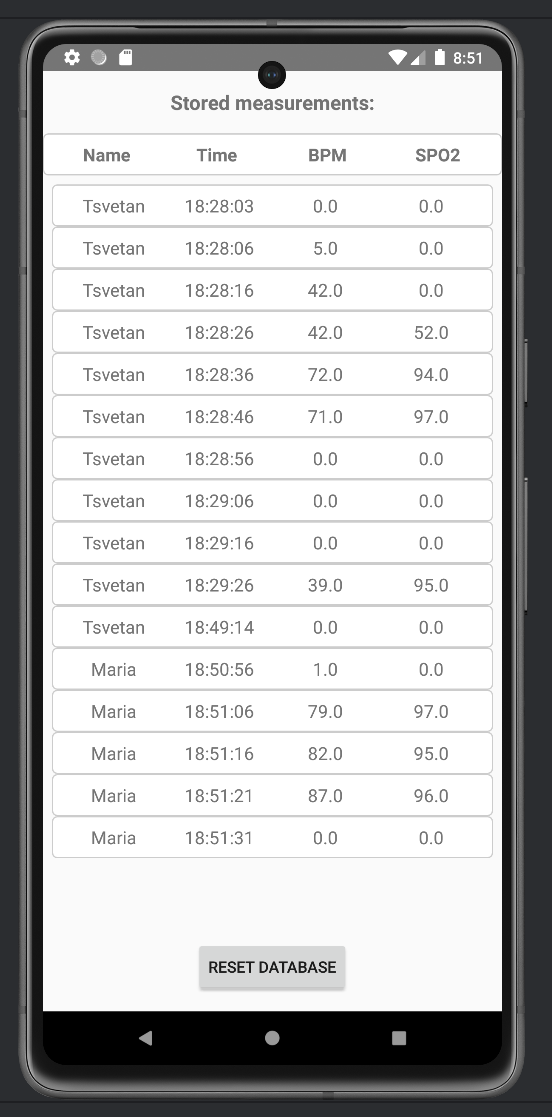
\includegraphics[width=0.4\textwidth]{db_visualization.png}
         \caption{Datenanzeigeseite}
         \label{fig:DB}
 \end{figure}
\textbf{Hauptverantwortlichkeiten:}
\begin{itemize}
    \vspace{0.5em}
    \item \textbf{Titel TextView:} Zeigt den Titel "Stored measurements" zentriert auf dem Bildschirm an. Der Titel gibt an, dass auf diesem Bildschirm die gespeicherten Messwerte angezeigt werden.
    \vspace{0.5em}
    \item \textbf{Datenanzeige-Liste:} Eine Liste, die die gespeicherten Messungen darstellt. Jede Zeile der Liste enthält den Namen des Benutzers, die Uhrzeit der Messung, den BPM (Herzfrequenz) und die SpO2-Werte. Die Liste ist so formatiert, dass die Daten klar und lesbar sind.
    \vspace{0.5em}
    \item \textbf{Datenbank zurücksetzen-Button:} Eine Schaltfläche zum Zurücksetzen der Datenbank. Der Button ist grau mit weißem Text und ist am unteren Rand des Bildschirms zentriert platziert. Durch das Drücken dieser Schaltfläche werden alle gespeicherten Daten gelöscht.
\end{itemize}

\subsubsection{Backend und Architekturüberblick}
Dieser UML-Diagramm gibt einen Überblick über unsere Backend-Architektur.\vspace{0.5em}\\
\begin{figure}[H]
         \centering
         \includesvg[width=0.5\textwidth]{uml.svg}
         \caption{UML-Klassendiagramm}
         \label{fig:funktionsnknoten-code}
\end{figure}
\underline{MainActivity}\vspace{0.5em}\\
MainActivity ist die zentrale Komponente der Anwendung. Sie verwaltet die Hauptbenutzeroberfläche, einschließlich Buttons und Textansichten, und interagiert mit anderen Komponenten, um wichtige Aufgaben auszuführen.\\

\textbf{Hauptverantwortlichkeiten:}
\begin{itemize}
    \vspace{0.5em}
    \item \textbf{Benutzeroberfläche:} Zeigt Herzfrequenz- und Sättigungswerte mithilfe von \texttt{heartRateTextView} und \texttt{satTextView} an. Außerdem bietet sie Buttons zum Starten und Stoppen der Datenerfassung, zum Anzeigen gespeicherter Daten und zum Aufrufen von Optionen.
    \vspace{0.5em}
    \item \textbf{Datenverwaltung:} Verwaltert eine Liste von Datenpunkten (\texttt{entries}) und aktualisiert das Diagramm (\texttt{lineChart}) mit neuen Daten.
    \vspace{0.5em}
    \item \textbf{MQTT-Verbindung:} Verwendet \texttt{MqttManager}, um eine Verbindung zu einem MQTT-Broker herzustellen, Nachrichten zu empfangen und diese angemessen zu verarbeiten.
    \vspace{0.5em}
    \item \textbf{Datenbankoperationen:} Nutzt \texttt{DatabaseHelper}, um Daten in der lokalen Datenbank zu speichern und abzurufen.
    \vspace{0.5em}
    \item \textbf{Soundmanagement:} Verwendet \texttt{SoundManager}, um basierend auf den Herzfrequenzdaten Töne abzuspielen.
    \vspace{0.5em}
\end{itemize}

\underline{ChartManager}\vspace{0.5em}\\
ChartManager ist verantwortlich für die Verwaltung der Anzeige von Daten in einem \texttt{LineChart}.\\

\textbf{Hauptverantwortlichkeiten:}
\begin{itemize}
    \vspace{0.5em}
    \item \textbf{Einrichten und Aktualisieren:} Initialisiert das Liniendiagramm und aktualisiert es mit neuen Datenpunkten.
    \vspace{0.5em}
    \item \textbf{Datenverwaltung:} Verwaltert eine Liste von \texttt{Entry}-Objekten und aktualisiert die \texttt{LineData} für das Diagramm.
    \vspace{0.5em}
\end{itemize}

\underline{DataAdapter}\vspace{0.5em}\\
DataAdapter wird verwendet, um eine Liste von \texttt{MqttData}-Objekten in einem \texttt{RecyclerView} zu verwalten und anzuzeigen.\\

\textbf{Hauptverantwortlichkeiten:}
\begin{itemize}
    \vspace{0.5em}
    \item \textbf{RecyclerView-Verwaltung:} Erstellt und bindet View-Holders, um die Datenpunkte anzuzeigen.
    \vspace{0.5em}
    \item \textbf{Datenbindung:} Bindet \texttt{MqttData}-Elemente an die Ansichten im \texttt{RecyclerView}.
    \vspace{0.5em}
\end{itemize}

\underline{DatabaseHelper}\vspace{0.5em}\\
DatabaseHelper verwaltet die Erstellung und Verwaltung der lokalen Datenbank.\\

\textbf{Hauptverantwortlichkeiten:}
\begin{itemize}
    \vspace{0.5em}
    \item \textbf{Datenbankoperationen:} Erstellt und aktualisiert die Datenbank. Außerdem bietet sie Methoden zum Einfügen neuer Daten, Abrufen aller Daten und Löschen aller Daten aus der Datenbank.
    \vspace{0.5em}
\end{itemize}

\underline{DataTableActivity}\vspace{0.5em}\\
DataTableActivity zeigt die gesammelten Daten in tabellarischer Form mithilfe eines \texttt{RecyclerView} an.\\

\textbf{Hauptverantwortlichkeiten:}
\begin{itemize}
    \vspace{0.5em}
    \item \textbf{UI-Verwaltung:} Initialisiert den \texttt{RecyclerView} und richtet den \texttt{DataAdapter} ein, um Daten anzuzeigen.
    \vspace{0.5em}
    \item \textbf{Datenbankinteraktion:} Verwendet \texttt{DatabaseHelper}, um Daten aus der Datenbank abzurufen und anzuzeigen.
    \vspace{0.5em}
\end{itemize}

\underline{MqttData}\vspace{0.5em}\\
MqttData ist eine Datenklasse, die einzelne Datenpunkte repräsentiert, die vom MQTT-Broker gesammelt wurden.\\

\textbf{Hauptverantwortlichkeiten:}
\begin{itemize}
    \item \textbf{Datenrepräsentation:} Enthält Attribute wie ID, Benutzername, Herzfrequenz (bpm), Sauerstoffsättigung (spo2) und Zeitstempel (dateTime). Bietet Getter- und Setter-Methoden für diese Attribute.
    \vspace{0.5em}
\end{itemize}

\underline{MqttManager}\vspace{0.5em}\\
MqttManager verwaltet die Verbindung zum MQTT-Broker und verarbeitet eingehende Nachrichten.\\

\textbf{Hauptverantwortlichkeiten:}
\begin{itemize}
    \vspace{0.5em}
    \item \textbf{Verbindungsmanagement:} Stellt eine Verbindung zum MQTT-Broker her und trennt diese wieder.
    \vspace{0.5em}
    \item \textbf{Nachrichtenverarbeitung:} Verarbeitet eingehende MQTT-Nachrichten und übergibt die Daten an \texttt{MainActivity} zur weiteren Verarbeitung.
    \vspace{0.5em}
\end{itemize}

\underline{OptionsActivity}\vspace{0.5em}\\
OptionsActivity ermöglicht es Benutzern, Anwendungseinstellungen wie den Benutzernamen zu konfigurieren.\vspace{3em}\\

\textbf{Hauptverantwortlichkeiten:}
\begin{itemize}
    \item \textbf{Einstellungsmanagement:} Bietet eine Benutzeroberfläche zur Eingabe und Speicherung des Benutzernamens mithilfe von \texttt{usernameEditText} und \texttt{saveButton}. Verwendet \texttt{SharedPreferences}, um diese Einstellungen zu speichern und abzurufen.
    \vspace{0.5em}
\end{itemize}

\underline{SoundManager}\vspace{0.5em}\\
SoundManager verwaltet die Wiedergabe von Tönen basierend auf den Herzfrequenzdaten.\vspace{0.5em}\\
\textbf{Hauptverantwortlichkeiten:}
\vspace{0.5em}
\begin{itemize}
    \item \textbf{Soundwiedergabe:} Spielt Töne ab, stoppt und gibt Ressourcen mithilfe eines \texttt{SoundPool} frei. Spielt einen Herzschlagton basierend auf dem aktuellen Herzfrequenzwert ab.
\end{itemize}

\underline{Wie alles zusammenarbeitet}\\
\begin{itemize}
    \item \textbf{Start:} Beim Start der App initialisiert \texttt{MainActivity} die Benutzeroberfläche und richtet Verbindungen zu verschiedenen Managern ein (\texttt{ChartManager}, \texttt{MqttManager}, \texttt{SoundManager} usw.).
    \vspace{0.5em}
    \item \textbf{Datenerfassung:} Beim Start der Datenerfassung stellt \texttt{MqttManager} eine Verbindung zum MQTT-Broker her und abonniert Themen für Herzfrequenz- und Sauerstoffsättigungsdaten.
    \vspace{0.5em}
    \item \textbf{Datenempfang:} Wenn Daten vom MQTT-Broker empfangen werden, übergibt \texttt{MqttManager} diese an \texttt{MainActivity}, die die Benutzeroberfläche aktualisiert und die Daten mithilfe von \texttt{DatabaseHelper} speichert.
    \vspace{0.5em}
    \item \textbf{Datenanzeige:} \texttt{MainActivity} aktualisiert das \texttt{LineChart} über \texttt{ChartManager}, um Echtzeitdaten anzuzeigen. Benutzer können detaillierte Daten in tabellarischer Form über \texttt{DataTableActivity} anzeigen.
    \vspace{0.5em}
    \item \textbf{Audiowiedergabe:} Basierend auf den Herzfrequenzdaten spielt \texttt{SoundManager} einen entsprechenden Ton ab, um akustisches Feedback zu geben.
    \vspace{0.5em}
    \item \textbf{Benutzereinstellungen:} Benutzer können Einstellungen wie ihren Benutzernamen in \texttt{OptionsActivity} konfigurieren, die mithilfe von \texttt{SharedPreferences} gespeichert werden.
\end{itemize}
\vspace{0.5em}
\section{Probleme und Diskussion}
Das erste Problem, das wir hatten, war mit dem Ton. Am Anfang des Dateiladens hört man ein Rauschen. Das könnte entweder an der Qualität der Datei liegen, die wir verwenden, oder am Ladevorgang selbst. Ein weiteres Problem ist, dass beim Neuladen des Diagramms in der Anwendung tatsächlich eine kleine Verzögerung auftritt. Aus diesem Grund geht manchmal eine der Messungen verloren und wird nicht korrekt visualisiert.
\clearpage
\section{Literatur}
\nocite{*} % This includes all entries from mucLiteratur.bib
\printbibliography % This prints the bibliography
\end{document}
